\chapter{Non-Negative Matrix Factorization}
This chapter introduces the NMF problem.
\section{Definition}
In its more general form the Non-negative matrix factorization problem can be defined as follows: given a non-negative matrix $V \in \R_+^{m \times n}$ and a factorization rank $r \in \N$ find two matrices
$W \in \R_+^{m \times r}$ and $H \in \R_+^{r \times n}$, constrained to be non-negative, such that their product $WH$ approximates $V$ as closely as possible according to some distance measure $D$.
\par
This problem can be formulated with an optimization problem as follows:
\begin{definition}[Non-Negative Matrix Factorization optimization problem]\label{NMF optimization problem}
Given a non-negative matrix $V \in \R_+^{m \times n}$ and a factorization rank $r \in \N$, find two non-negative matrices $W \in \R_+^{m \times r}$ and $H \in \R_+^{r \times n}$ that minimize 
a given cost function $D(V, WH)$, that is:
\begin{equation}
\min_{W \in \R_+^{m \times r}, H \in \R_+^{r \times n}} D(V, WH)
\end{equation}
where $D$ is a distance measure between matrices.
\end{definition}
\section{Metrics}
Some introduction here ...
\subsection{Frobenius norm}
Probably the most common choice for the distance measure $D$ in the NMF problem \ref{NMF optimization problem} is the squared Frobenius norm:
\begin{equation}
    D(V, WH) = ||V - WH||_F^2 = \sum_{i=1}^{m} \sum_{j=1}^{n} (V[i,j] - (WH)[i,j])^2
\end{equation}
This choice leads to the following optimization problem:
\begin{equation}
    \min_{W \in \R_+^{m \times r}, H \in \R_+^{r \times n}} ||V - WH||_F^2
\end{equation}
A justification for the use of Frobenius norm as objective function of the optimization problem \ref{NMF optimization problem} can be given from a statistical point of view.
The Frobenius norm can be obtained using the principle of maximum likelihood estimation assuming that the elements of the matrix $V$ are affected by a i.i.d. Gaussian noise.
See \cite{gillis2020nonnegative} chapter $5.1$.
\par
Suppose that each element of $V$ is generated as:
\begin{equation}
    V[i,j] = (WH)[i,j] + \epsilon_{i,j}
\end{equation}
where $\epsilon_{i,j} \sim \mathcal{N}(0, \sigma^2)$ are i.i.d. Gaussian noise variables with zero mean and variance $\sigma^2$.
The likelihood of observing the matrix $V$ given the parameters $W$ and $H$ is:
\begin{equation}
    L(WH ; V) = \prod_{i=1}^{m} \prod_{j=1}^{n} \frac{1}{\sqrt{2 \pi \sigma^2}} \exp\left(-\frac{(V[i,j] - (WH)[i,j])^2}{2 \sigma^2}\right)
\end{equation}
The log-likelihood $\ell(WH ; V) = \log L(WH ; V)$  is:
\begin{equation}
    \ell(WH ; V) =  -\frac{mn}{2} \log(2 \pi \sigma^2) - \frac{1}{2 \sigma^2} \sum_{i=1}^{m} \sum_{j=1}^{n} (V[i,j] - (WH)[i,j])^2
\end{equation}
Maximizing the log-likelihood 
\begin{equation}
    \max_{W \in \R_+^{m \times r}, H \in \R_+^{r \times n}} \ell(WH ; V)
\end{equation}
is equivalent to minimizing the sum of squared errors:
\begin{equation}
    \min_{W \in \R_+^{m \times r}, H \in \R_+^{r \times n}} \sum_{i=1}^{m} \sum_{j=1}^{n} (V[i,j] - (WH)[i,j])^2
\end{equation}
which is exactly the Frobenius norm.
\par
\subsection{Kullback-Leibler}
Another popular choice for the distance measure $D$ in the NMF problem \ref{NMF optimization problem} is the Kullback-Leibler (KL) divergence:
\begin{equation}
    D(V, WH) = D_{KL}(V \| WH) = \sum_{i=1}^{m} \sum_{j=1}^{n} \left( V[i,j] \log \frac{V[i,j]}{(WH)[i,j]} - V[i,j] + (WH)[i,j] \right) 
\end{equation}
This choice leads to the following optimization problem:
\begin{equation}
    \min_{W \in \R_+^{m \times r}, H \in \R_+^{r \times n}} D_{KL}(V \| WH)
\end{equation}
As with the Frobenius norm, we can use the maximum likelihood principle to obtain the KL divergence as objective function of the NMF problem \ref{NMF optimization problem} assuming that the elements of the matrix $V$ are affected by a i.i.d. Poisson noise.
See \cite{gillis2020nonnegative} 5.1.1.
\subsection{$\beta$-divergence}
The $\beta$-divergence is a family of cost functions that generalizes both the Frobenius norm and the Kullback-Leibler divergence.
It is defined as follows:
\begin{equation}
    D_{\beta}(V, WH) = \sum_{i=1}^{m} \sum_{j=1}^{n} d_{\beta}(V[i,j], (WH)[i,j])
\end{equation}
where 
\begin{equation}
    d_{\beta}(x,y) = \begin{cases}
        \frac{x}{y} - \log \frac{x}{y} - 1 & \text{if } \beta = 0 \\
        x \log \frac{x}{y} - x + y & \text{if } \beta = 1 \\
        \frac{1}{\beta(\beta - 1)}\left(x^\beta + (\beta - 1)y^\beta - \beta x y^{\beta - 1}\right) & \text{if } \beta \neq 0, 1
    \end{cases}
\end{equation}
It easy to show that for $\beta = 2$ the $\beta$-divergence reduces to the squared Frobenius norm and for $\beta = 1$ it reduces to the Kullback-Leibler divergence.
The case where $\beta = 0$ is known as the Itakura-Saito divergence\footnote{\href{https://en.wikipedia.org/wiki/Itakura\%E2\%80\%93Saito\_distance}{https://en.wikipedia.org/wiki/Itakura Saito distance}}.
\begin{figure}[h]
    \centering
    \includegraphics[width=1.0\textwidth]{Imgs/Beta_diveregence_plot.png}
    \caption{Plot of the $\beta$-divergence for $\beta$ values of $0$, $1$ $\frac{1}{2}$, $2$, and $3$.}
    \label{beta_divergence_plot}
\end{figure}

The choice of the $\beta$-divergence as objective function leads to the following optimization problem:
\begin{equation}
    \min_{W \in \R_+^{m \times r}, H \in \R_+^{r \times n}} D_{\beta}(V, WH)
\end{equation}

\section{Complexity of NMF}
The main result was proved by Vavasis in \cite{vavasis2007complexitynonnegativematrixfactorization} where it is shown that the NMF problem is NP-hard in general.
To do so Vavasis considers the exact NMF problem, a particular case of NMF where the distance measure is such that $D(V, WH) = 0$ if and only if $V = WH$ and $D(V, WH) > 0$ otherwise.
\begin{definition}[Exact Non-Negative Matrix Factorization problem]\label{Exact NMF definition}
      Given a nonnegative matrix $V \in \R^{m\times n}_+$ and a factorization rank $r$,
compute, if possible, two nonnegative matrices
$W \in \R^{m \times r}_+$ and $H \in \R^{r \times n}_+$
such that
\begin{equation}
    V = WH
\end{equation}
The pair $(W , H)$ is said to be an Exact NMF of $V$ of size $r$.  
\end{definition}
Behind every approximation $\tilde{V}\approx WH$ an exact NMF is hidden.
Exact NMF has a nice \textit{geometric interpretation} which allows one to
characterize the set of solutions.   
\par
Since the NMF problem as stated in \ref{NMF optimization problem} is a generalization of the exact NMF problem, the NP-hardness of exact NMF implies the NP-hardness of NMF.
\section{Identifiability}
Let's start with an observation: In the case of the exact factorization $V = WH$, if we consider any invertible matrix $Q \in \R^{r \times r}$ such that both $WQ$ and $Q^{-1}H$ are non-negative matrices, then we have another exact factorization of $V$ given by:
\begin{equation}
    V = WH = (WQ)(Q^{-1}H)
\end{equation}
This simple observation shows that in general the NMF problem does not have a unique solution.
\par
Even after removing this scaling ambiguity, one should not expect to find an unique NMF solution in general.
in the literature this is also known as the \textit{identifiability} problem of NMF. See \cite{gillis2020nonnegative} chapter $4$ for a detailed discussion on this topic.
\par
In this section we will observe which necessary condition is required for identifiability and present a sufficient condition for identifiability.
To do so we first need the definition of the \textit{support} of a vector.
\begin{definition}[Support of a vector]
Given a vector $x \in \R^n$, the support of $x$ is defined as:
\begin{equation}
    \text{supp}(x) = \{ i \in \{1, \ldots, n\} | x_i \neq 0 \}
\end{equation}
\end{definition}
The next theorem states that a necessary condition for identifiability is that the support of any column of W does not contain the support of any other column of W
\begin{theorem}
[Necessary condition for identifiability]\label{Necessary condition for identifiability}
Let $V \in \R_+^{m \times n}$ be a non-negative matrix and let $V = WH$ be an exact NMF of $V$ of size $r$.
If the exact NMF of $V$ is unique (up to scaling and permutation) then for any pair of distinct columns $W[:,i]$ and $W[:,j]$ of $W$ it holds that:
\begin{equation}
    \text{supp}(W[:,i]) \nsubseteq \text{supp}(W[:,j])
\end{equation} 
\end{theorem}
\begin{proof}
Assume by contradiction that there exist two distinct columns $W[:,i]$ and $W[:,j]$ of $W$ such that:
\begin{equation}
    \text{supp}(W[:,i]) \subseteq \text{supp}(W[:,j])
\end{equation}
Then we can construct a new pair of matrices $(\tilde{W}, \tilde{H})$ as follows:
\begin{equation}
    \tilde{W}[:,k] = 
    \begin{cases}
        W[:,k] & \text{if } k \neq j \\
        W[:,j] + \alpha W[:,i] & \text{if } k = j
    \end{cases}
\end{equation}
\begin{equation}
    \tilde{H}[k,:] = 
    \begin{cases}
        H[k,:] & \text{if } k \neq i \\
        H[i,:] - \alpha H[j,:] & \text{if } k = i
    \end{cases}
\end{equation} 
such that $W[:,j] + \alpha W[:,i] \geq 0$ and $H[i,:] - \alpha H[j,:] \geq 0$ for some $\alpha > 0$.
It is easy to see that $(\tilde{W}, \tilde{H})$ is another exact NMF of $V$ of size $r$:
\begin{equation}
    \tilde{W} \tilde{H} = W H = V
\end{equation}
This contradicts the assumption that the exact NMF of $V$ is unique.
\end{proof}
Now we present a sufficient condition for identifiability known as the \textit{separability} condition.
\begin{theorem}
[Sufficient condition for identifiability: Separability]\label{Sufficient condition for identifiability}
Let $V \in \R_+^{m \times n}$ be a non-negative matrix and let $V = WH$ be an exact NMF of $V$ of size $r$.
The matrices $W$ and $H$ contain non-singular diagonal submatrices of size $r \times r$, then the NMF solutions are identifiable.
\end{theorem}
\begin{proof}
    The properties of separable matrices are analyzed in \cite{donoho2003does}.
\end{proof}
An equivalent definition of separability is the following:
\begin{definition}[Separable NMF]
An NMF $V = WH$ is said to be separable if there exists a set of indices $\{j_1, j_2, \ldots, j_r\} \subseteq \{1, 2, \ldots, n\}$ of size $r$ such that:
\begin{equation}
    V = W H = V[:, \{j_1, j_2, \ldots, j_r\}]\tilde{H}
\end{equation}
\end{definition}
\begin{figure}[h]
\centering
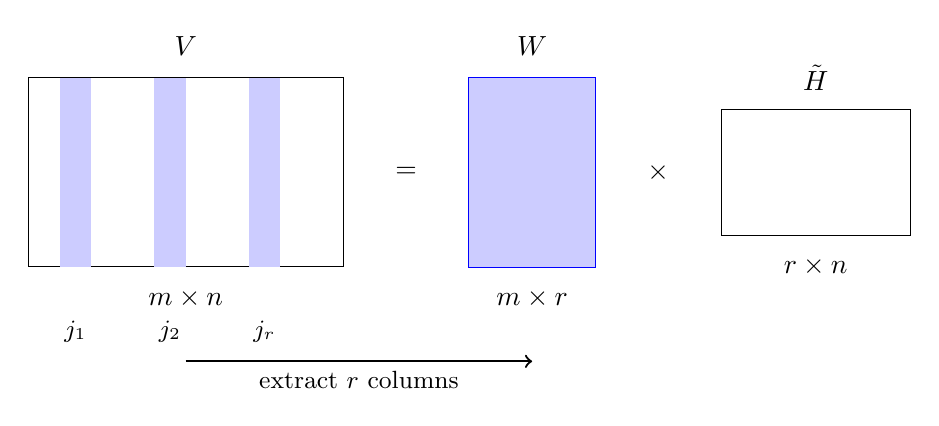
\begin{tikzpicture}[scale=0.8]
    % Matrix V
    \draw (0,0) rectangle (5,3);
    \node at (2.5,3.5) {$V$};
    \node at (2.5,-0.5) {$m \times n$};
    
    % Highlight selected columns
    \fill[blue!20] (0.5,0) rectangle (1,3);
    \fill[blue!20] (2,0) rectangle (2.5,3);
    \fill[blue!20] (3.5,0) rectangle (4,3);
    
    % Column labels
    \node[below] at (0.75,-0.7) {\small $j_1$};
    \node[below] at (2.25,-0.7) {\small $j_2$};
    \node[below] at (3.75,-0.7) {\small $j_r$};
    
    % Equals sign
    \node at (6,1.5) {$=$};
    
    % Matrix W (selected columns of V)
    \draw[thick,blue] (7,0) rectangle (9,3);
    \node at (8,3.5) {$W$};
    \node at (8,-0.5) {$m \times r$};
    \fill[blue!20] (7,0) rectangle (9,3);
    
    % Times sign
    \node at (10,1.5) {$\times$};
    
    % Matrix H-tilde
    \draw (11,0.5) rectangle (14,2.5);
    \node at (12.5,3) {$\tilde{H}$};
    \node at (12.5,0) {$r \times n$};
    
    % Arrow showing extraction
    \draw[->,thick,black] (2.5,-1.5) -- (8,-1.5);
    \node[below] at (5.25,-1.5) {\small extract $r$ columns};
\end{tikzpicture}
\caption{Visualization of separable NMF: the matrix $W$ consists of $r$ selected columns from $V$, indexed by $\{j_1, j_2, \ldots, j_r\}$.}
\label{fig:separable_nmf}
\end{figure}
The separable matrices represent an important class of matrices in applications \cite{arora2012computing}, \cite{gillis2013fast}; for example in text mining \cite{arora2013practical}, 
hyperspectral imaging \cite{boardman1995mapping}, and for some computer vision tasks like background-foreground separation \cite{kumar2015near}.
\par
There are other sufficient conditions that are not included in this thesis, the interested reader may refer to \cite{huang2013non} for a geometrical perspective on uniqueness results.
\section{Geometric Interpretation}
The aim of this section is to provide a geometric intuition on the NMF problem and provide references to the existent literature that adresses this topic.
This topic is extremely vast therefore in this section only a brief overview is given.
\subsection{Linear dimensionality reduction interpretation}
A way to interpret NMF is that we are seeking a representation of the data points (columns of $V$) as non-negative linear combinations of basis elements (columns of $W$).
That is we wish to find $r$ basis vectors (columns of $W$) such that each data point (column of $V$) can be expressed as a non-negative linear combination of these basis vectors weighted by the coefficients in the corresponding column of $H$.
\begin{equation}
    V[:,j] \approx WH[:,j] = \sum_{k=1}^{r} H[k,j] W[:, k] \quad \forall j = 1, \ldots, n
\end{equation}
% todo add visualization

\begin{figure}[h]
\centering
\begin{tikzpicture}[scale=1.3, >=Stealth]
    %  2. Coordinate Definitions
    \coordinate (O) at (0,0);       % Origin
    \coordinate (W1) at (1.8, 2.5); % Vector 1 (Left/Up)
    \coordinate (W2) at (3.0, 1.2); % Vector 2 (Right)
    
    % Define the "Cone" / Subspace
    \coordinate (TopRight) at ($(W1)+(W2)!1.5!(W2)$); % Extrapolation
    \coordinate (FarPoint) at (8, 5.5); % Just a reference
    
    %  3. The Gray Subspace (Cone) 
    % Drawing the filled gray area bounded by W1 and W2
    \fill[gray!40] (O) -- (W1) -- (5.5, 4.5) -- (8, 5.2) -- (W2) -- cycle;

    % 4. Basis Vectors 
    \draw[->, thick, red] (O) -- (W1) node[midway, left, xshift=-2pt] {\large $W(:,1)$};
    \draw[->, thick, red] (O) -- (W2) node[midway, below, yshift=-2pt] {\large $W(:,2)$};

    %  5. Data Points (The 'x' markers) 
    \foreach \p in {
        (1.2, 1.8), (1.5, 2.0), (1.6, 1.2), (2.0, 2.5), (2.2, 1.8),
        (2.5, 3.0), (2.8, 2.2), (3.0, 3.5), (3.2, 1.5), (3.5, 2.8),
        (4.0, 3.2), (4.2, 4.0), (4.5, 3.5), (5.0, 4.2), (5.5, 4.8),
        (1.0, 0.8), (2.5, 1.0), (3.5, 2.0), (4.5, 2.5), (5.8, 3.0),
        (7.0, 5.0), (7.5, 5.3), (6.0, 4.5), (3.0, 4.0), (2.0, 3.5),
        (2.5, 1.5), (3.8, 2.2), (4.8, 3.8), (1.8, 1.0), (0.5, 0.5)
    } {
        \fill[blue] \p circle (2.0pt);
    }

    %  6. Legend (In-plot) 
    \fill[blue] (1.0, 5.0) circle (2.0pt) node[right, xshift=5pt] {\small Data Points (Columns of $V$)};

    %  7. Origin 
    \fill[red] (O) circle (2pt);
    \node[red, anchor=north east, font=\large\bfseries] at (0,0) {0};

    %  8. Mini Coordinate System (Bottom Right Inset) 
    \begin{scope}[shift={(6.5, 0.5)}, scale=0.4]
        \draw[->] (0,0) -- (0,2); % z
        \draw[->] (0,0) -- (1.5,0); % y
        \draw[->] (0,0) -- (-1,-1); % x
    \end{scope}
\end{tikzpicture}
\caption{NMF seeks a low-dimensional non-negative subspace (gray area) spanned by basis vectors (black arrows) such that data points (blue dots) lie close to this subspace. Each data point can be approximated as a non-negative linear combination of the basis vectors.}
\label{fig:dimensionality_reduction interpretation}
\end{figure}
In this sense NMF can be thought of as a linear dimensionality reduction technique for matrices of non-negative data.
\subsection{Geometric interpretation with cones}
We begin by giving a definition of convex cone.
\begin{definition}[Convex cone]
A set $C \subseteq \R^m$ is a convex cone if for any $x, y \in C$ and any non-negative scalars $\alpha, \beta \geq 0$ it holds that:
\begin{equation}
    \alpha x + \beta y \in C
\end{equation}
\end{definition}
Given a matrix $A \in \R^{m \times n}$, the convex cone generated by the columns of $A$ is defined as:
\begin{equation}
    \text{cone}(A) = \{ Ax | x \in \R_+^{n} \}
\end{equation}
\begin{observation}
    $dim(\text{cone}(A)) = rank(A)$
\end{observation}
As seen in [add reference here] the $j$-th column of $V$ can be expressed as:
\begin{equation}
    V[:,j] = WH[:,j] \ \forall j = 1, \ldots, n
\end{equation}
This means that each column of $V$ lies in the convex cone generated by the columns of $W$.
In other words:
\begin{equation}
    \text{cone}(V) \subseteq \text{cone}(W)
\end{equation}
% Figure \ref{fig:cone_interpretation} illustrates this concept in two dimensions with $r = 3$.
\par
\begin{figure}[h]
\centering
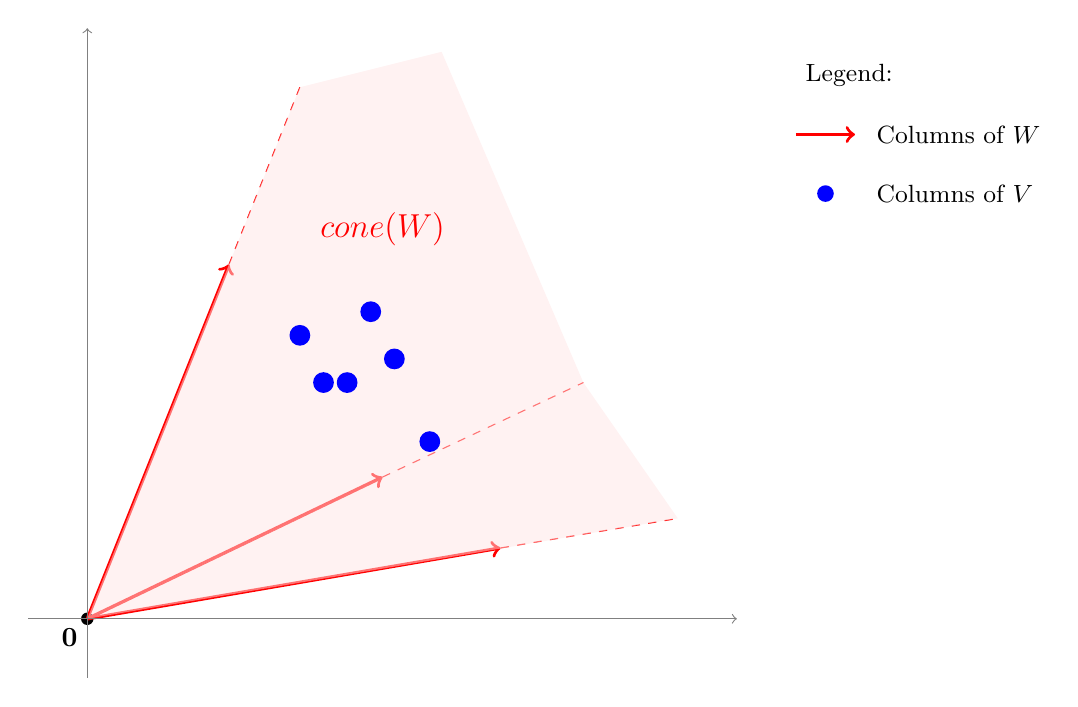
\begin{tikzpicture}[scale=1.5]
    % Origin
    \coordinate (O) at (0,0);
    \fill (O) circle (1.5pt);
    \node[below left] at (O) {$\mathbf{0}$};
    
    % Columns of W (basis vectors)
    \draw[->,very thick,red] (O) -- (2.5,1.2) coordinate (W1);
    \draw[->,very thick,red] (O) -- (1.2,3) coordinate (W2);
    \draw[->,very thick,red] (O) -- (3.5,0.6) coordinate (W3);
    
    % Cone boundary (dashed lines extending the basis)
    \draw[dashed,red,thin] (W1) -- (4.2,2);
    \draw[dashed,red,thin] (W2) -- (1.8,4.5);
    \draw[dashed,red,thin] (W3) -- (5,0.85);
    
    % Shaded cone region
    \fill[red!10,opacity=0.5] (O) -- (4.2,2) -- (3,4.8) -- (1.8,4.5) -- cycle;
    \fill[red!10,opacity=0.5] (O) -- (4.2,2) -- (5,0.85) -- cycle;
    
    % Label for cone(W)
    \node[red,font=\large] at (2.5,3.3) {$\text{cone}(W)$};
    
    % Columns of V (data points inside the cone)
    \fill[blue] (2.2,2.0) circle (2.5pt);
    \fill[blue] (2.6,2.2) circle (2.5pt);
    \fill[blue] (1.8,2.4) circle (2.5pt);
    \fill[blue] (2.9,1.5) circle (2.5pt);
    \fill[blue] (2.4,2.6) circle (2.5pt);
    \fill[blue] (2.0,2.0) circle (2.5pt);
    
    % Axes (for reference)
    \draw[->,thin,gray] (-0.5,0) -- (5.5,0);
    \draw[->,thin,gray] (0,-0.5) -- (0,5);
    
    % Legend box
    \begin{scope}[shift={(6,3.5)}]
        % \draw[thick] (-0.3,-0.3) rectangle (2.8,1.5);
        \node[anchor=west] at (0,1.1) {\small Legend:};
        
        \draw[->,very thick,red] (0,0.6) -- (0.5,0.6);
        \node[anchor=west] at (0.6,0.6) {\small Columns of $W$};
        
        \fill[blue] (0.25,0.1) circle (2pt);
        \node[anchor=west] at (0.6,0.1) {\small Columns of $V$};
    \end{scope}
\end{tikzpicture}
\caption{Geometric interpretation: each column of $V$ (blue points) is a non-negative linear combination of the columns of $W$ (red vectors), meaning $V[:,j] = \sum_{k=1}^{r} H[k,j] W[:,k]$. All columns of $V$ lie in the convex cone generated by the columns of $W$.}
\label{fig:cone_interpretation}
\end{figure}
% TODO: add references to literature on geometric interpretation of NMF
Often in the literature the geometric interpretation of NMF is analyzed in terms of nested polytopes.
The reason for this is that because it is easier to visualize and because there is a close connection between the NMF problem in computational geometry known as the and the nested polytope problem (NPP) \cite{shitov2018universalitytheoremnonnegativematrix} \cite{donoho2003does}.
For an overview on the NPP see: \cite{dobbins2019universalitytheoremnestedpolytopes}.
A detailed discussion on the geometric interpretation of NMF can be found in \cite{gillis2020nonnegative} chapter $2.1$.
An example with nested hexagons can be found in \cite{gillis2017introductionnonnegativematrixfactorization}.

\section{Historical origin of NMF}
Even though some early works date back to the 60s in the field of Earth science and remote system sensing \cite{Wallace1960}\cite{Imbrie1964}\cite{craig1994}
the first modern definition of the NMF problem is usually attributed to the work of Paatero and Tapper in 1994 \cite{Paatero1994} where they defined the so-called Positive Matrix Factorization (PMF) problem, a particular case of NMF where the distance measure used is the least squares one (Frobenius norm).
This early work arose in the field of analytical chemistry and the NMF model as a modern data analysis tool remained relatively unknown until the seminal paper of Lee and Seung in 1999 \cite{Lee1999}.
\par
In their work Lee and Seung introduce the NMF model to the machine learning community and proposed an easy to implement algorithm based on multiplicative updates to find local minima of the NMF optimization problem \ref{NMF optimization problem}.
Their work is especially famous because they  demonstrate an algorithm for non-negative matrix factorization that is able to learn parts of faces, in contrast to other decomposition methods like PCA or SVD that learn holistic features.
Their results are also reproduced in this thesis in section \ref{Example feature extraction NMF} to show a prominent example of NMF's application.
\section{Two applications of NMF}
In this section two applications of NMF are presented: the first one is the well-known example of learning parts of faces introduced by Lee and Seung in \cite{Lee1999},
while the second one is an application of NMF to text mining, in particular to topic modeling.
\subsection{Learning parts of faces} \label{Example feature extraction NMF}
The dataset used in this example is the CBCL face dataset \footnote{See \ref{code documentation appendix} for data availability and details on the code used}.
This dataset has size $2429 \times 361$ where each column represent a $19 \times 19$ gray-scale image of a face.
\begin{figure}[h]
    \centering
    \includegraphics[width=0.5\textwidth]{Imgs/CBCL_Original.png}
    \caption{Some example images from the CBCL face dataset.}
    \label{fig:CBCL original faces}
\end{figure}
The NMF model is applied to this dataset with a factorization rank of $r = 49$,  the algorithm used is the multiplicative updates with the Kullback-Leibler divergence as distance measure.
After fitting the model we obtain two matrices: $W \in \R_+^{2429 \times 49}$ and $H \in \R_+^{49 \times 361}$.
The non-negativity constraints of the NMF problem \ref{NMF optimization problem} allows one to interpret the columns of $W$ in the same way as the original data, that is each column of $W$ can be reshaped to form a $19 \times 19$ gray-scale image and displayed.
\begin{figure}[h]
    \centering
    \includegraphics[width=0.75\textwidth]{Imgs/CBCL_colums_of_W.png}
    \caption{Columns of the matrix $W$ reshaped as $19 \times 19$ gray-scale images.}
    \label{fig:CBCL columns of W}
\end{figure}
As can be seen in figure \ref{fig:CBCL columns of W} the pixels of the images formed by the columns of $W$ are active only in certain regions, for example some columns represent eyes, others noses, mouths and so on.
This is the reason why it is said that Non-negative matrix factorization is able to learn a ``part based'' representation of faces.
\par
The matrix $H$ contains the coefficients or weights to reconstruct the original images as linear combinations of the parts.\\
The $j$-th column of the original data matrix $V$ can be approximated as:
\begin{equation}
    V[:,j] \approx W H[:,j] = \sum_{k=1}^{r} H[k,j] W[:, k]
\end{equation}
This is a linear combination of the columns of $W$ weighted by the coefficients in the $j$-th column of $H$.
\begin{equation}
    \begin{bmatrix}
        v_{1,j} \\
        v_{2,j} \\
        \vdots \\
        v_{m,j}
    \end{bmatrix} \approx H[1,j]
    \begin{bmatrix}
        w_{1,1} \\
        w_{2,1} \\
        \vdots \\
        w_{m,1}
    \end{bmatrix} + H[2,j]
    \begin{bmatrix}
        w_{1,2} \\
        w_{2,2} \\
        \vdots \\
        w_{m,2}
    \end{bmatrix} + \ldots + H[r,j]
    \begin{bmatrix}
        w_{1,r} \\
        w_{2,r} \\
        \vdots \\
        w_{m,r}
    \end{bmatrix}
\end{equation}
Note that the number of columns of $V$ is equal to the number of columns of $H$. That means that there is a one-to-one correspondence between the columns of $V$ and the columns of $H$ containing the weights to reconstruct each image.
\begin{figure}[h]
    \centering
    \includegraphics[width=0.5\textwidth]{Imgs/Reconstruction_1.png}
    \caption{Example of reconstruction of an image from the CBCL dataset using the NMF model. On the left the original image, on the right the reconstructed one.}
    \label{fig:CBCL reconstructed faces}
\end{figure}
\subsection{Topic modeling}
TODO